% Options for packages loaded elsewhere
\PassOptionsToPackage{unicode}{hyperref}
\PassOptionsToPackage{hyphens}{url}
\PassOptionsToPackage{space}{xeCJK}
\documentclass[
  10pt,
]{article}
\usepackage{xcolor}
\usepackage[margin=0.8in]{geometry}
\usepackage{amsmath,amssymb}
\setcounter{secnumdepth}{-\maxdimen} % remove section numbering
\usepackage{iftex}
\ifPDFTeX
  \usepackage[T1]{fontenc}
  \usepackage[utf8]{inputenc}
  \usepackage{textcomp} % provide euro and other symbols
\else % if luatex or xetex
  \usepackage{unicode-math} % this also loads fontspec
  \defaultfontfeatures{Scale=MatchLowercase}
  \defaultfontfeatures[\rmfamily]{Ligatures=TeX,Scale=1}
\fi
\usepackage{lmodern}
\ifPDFTeX\else
  % xetex/luatex font selection
  \setmainfont[]{Arial}
  \ifXeTeX
    \usepackage{xeCJK}
    \setCJKmainfont[]{Microsoft YaHei}
  \fi
  \ifLuaTeX
    \usepackage[]{luatexja-fontspec}
    \setmainjfont[]{Microsoft YaHei}
  \fi
\fi
% Use upquote if available, for straight quotes in verbatim environments
\IfFileExists{upquote.sty}{\usepackage{upquote}}{}
\IfFileExists{microtype.sty}{% use microtype if available
  \usepackage[]{microtype}
  \UseMicrotypeSet[protrusion]{basicmath} % disable protrusion for tt fonts
}{}
\makeatletter
\@ifundefined{KOMAClassName}{% if non-KOMA class
  \IfFileExists{parskip.sty}{%
    \usepackage{parskip}
  }{% else
    \setlength{\parindent}{0pt}
    \setlength{\parskip}{6pt plus 2pt minus 1pt}}
}{% if KOMA class
  \KOMAoptions{parskip=half}}
\makeatother
\usepackage{longtable,booktabs,array}
\newcounter{none} % for unnumbered tables
\usepackage{calc} % for calculating minipage widths
% Correct order of tables after \paragraph or \subparagraph
\usepackage{etoolbox}
\makeatletter
\patchcmd\longtable{\par}{\if@noskipsec\mbox{}\fi\par}{}{}
\makeatother
% Allow footnotes in longtable head/foot
\IfFileExists{footnotehyper.sty}{\usepackage{footnotehyper}}{\usepackage{footnote}}
\makesavenoteenv{longtable}
\usepackage{graphicx}
\makeatletter
\newsavebox\pandoc@box
\newcommand*\pandocbounded[1]{% scales image to fit in text height/width
  \sbox\pandoc@box{#1}%
  \Gscale@div\@tempa{\textheight}{\dimexpr\ht\pandoc@box+\dp\pandoc@box\relax}%
  \Gscale@div\@tempb{\linewidth}{\wd\pandoc@box}%
  \ifdim\@tempb\p@<\@tempa\p@\let\@tempa\@tempb\fi% select the smaller of both
  \ifdim\@tempa\p@<\p@\scalebox{\@tempa}{\usebox\pandoc@box}%
  \else\usebox{\pandoc@box}%
  \fi%
}
% Set default figure placement to htbp
\def\fps@figure{htbp}
\makeatother
\setlength{\emergencystretch}{3em} % prevent overfull lines
\providecommand{\tightlist}{%
  \setlength{\itemsep}{0pt}\setlength{\parskip}{0pt}}
\usepackage{bookmark}
\IfFileExists{xurl.sty}{\usepackage{xurl}}{} % add URL line breaks if available
\urlstyle{same}
\hypersetup{
  hidelinks,
  pdfcreator={LaTeX via pandoc}}

\author{}
\date{}

\usepackage{float}
\begin{document}

\section{Model training progress}\label{model-training-progress}

English \textbar{} \href{训练进展报告.md}{中文}

Reviewed November 12, 2026. This report describes saved training and model-validation records. It complements the \href{../2026-11-11/eye_sentinel_full_progress_20261111_en.pdf}{November 11 project progress report}.

\subsection{Training and data}\label{training-and-data}

{\def\LTcaptype{none} % do not increment counter
\begin{longtable}[]{@{}
  >{\raggedright\arraybackslash}p{(\linewidth - 8\tabcolsep) * \real{0.1667}}
  >{\raggedright\arraybackslash}p{(\linewidth - 8\tabcolsep) * \real{0.1667}}
  >{\raggedleft\arraybackslash}p{(\linewidth - 8\tabcolsep) * \real{0.2222}}
  >{\raggedleft\arraybackslash}p{(\linewidth - 8\tabcolsep) * \real{0.2222}}
  >{\raggedleft\arraybackslash}p{(\linewidth - 8\tabcolsep) * \real{0.2222}}@{}}
\toprule\noalign{}
\begin{minipage}[b]{\linewidth}\raggedright
Task
\end{minipage} & \begin{minipage}[b]{\linewidth}\raggedright
Model
\end{minipage} & \begin{minipage}[b]{\linewidth}\raggedleft
Training / validation images
\end{minipage} & \begin{minipage}[b]{\linewidth}\raggedleft
Epochs completed
\end{minipage} & \begin{minipage}[b]{\linewidth}\raggedleft
Training steps
\end{minipage} \\
\midrule\noalign{}
\endhead
\bottomrule\noalign{}
\endlastfoot
Glaucoma A & EfficientNet-B0 & 10,354 / 1,190 & 20 / 20 & 12,960 \\
Glaucoma B, candidate & ResNet50 & 10,354 / 1,190 & 20 / 20 & 12,960 \\
Original quality model & EfficientNet-B0 & 12,147 / 1,642 & 20 / 20 & 15,200 \\
EyeQ quality model & EfficientNet-B0 & 4,722 / 616 & 20 / 20 & 5,920 \\
\end{longtable}
}

\begin{figure}[H]
\centering
\pandocbounded{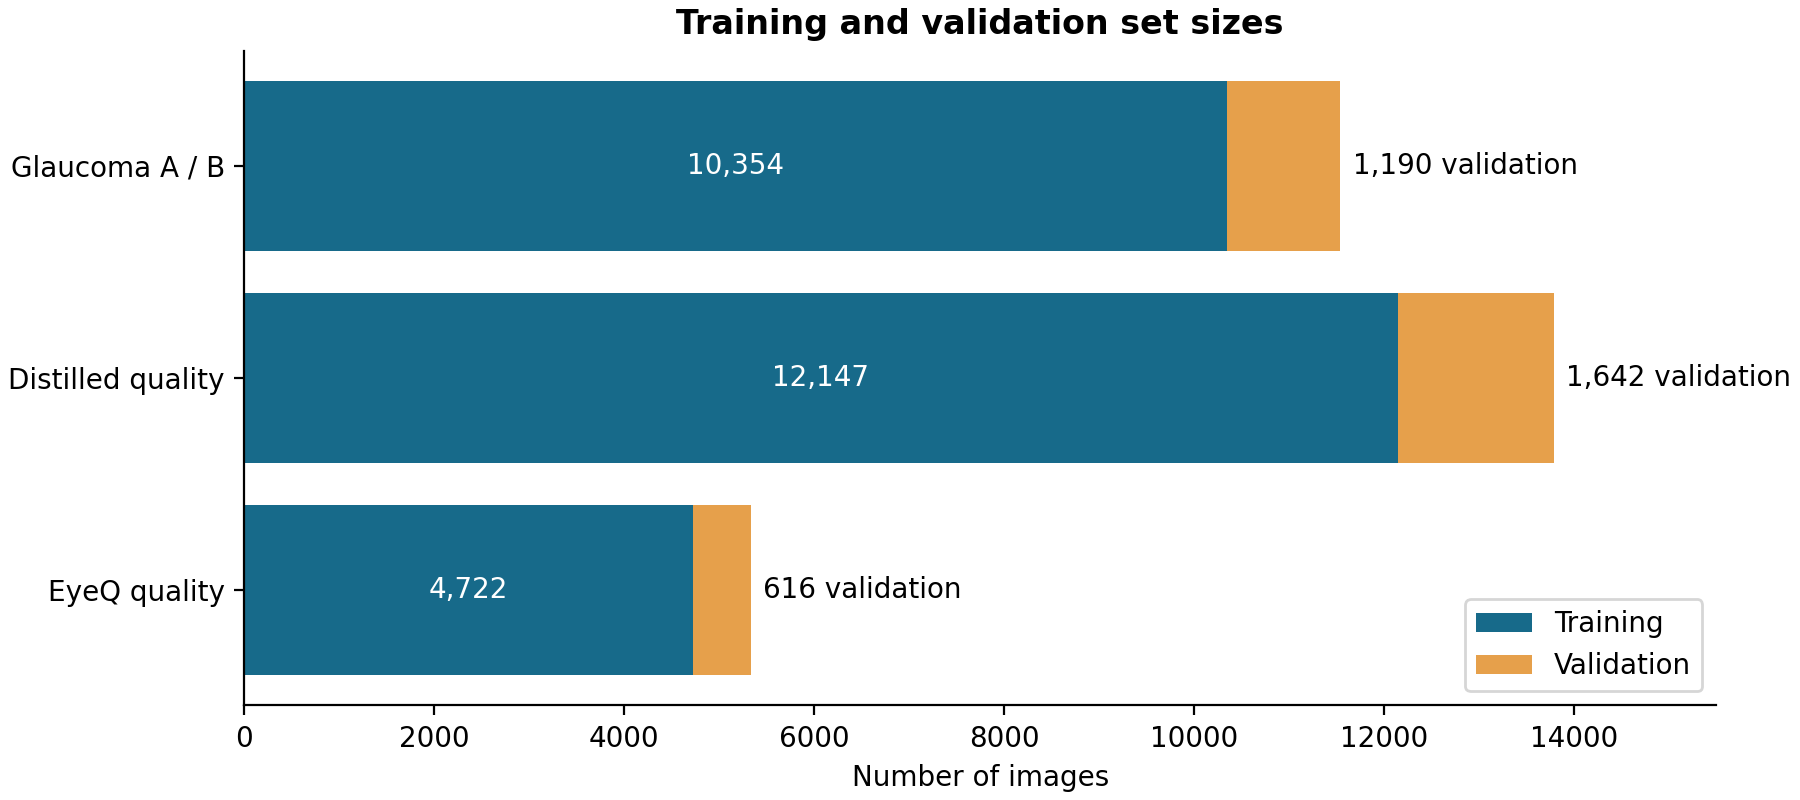
\includegraphics[keepaspectratio,alt={Training and validation set sizes}]{07_dataset_sizes.png}}
\caption{Training and validation set sizes}
\end{figure}

Both training pipelines report completion. An epoch is one pass through the training data; a step uses one batch of images to update the model. The two glaucoma models use the same data split. Each run records a loss at every training step and validation results after each epoch. Loss measures the difference between model output and its training target; lower is better for that target.

\begin{figure}[H]
\centering
\pandocbounded{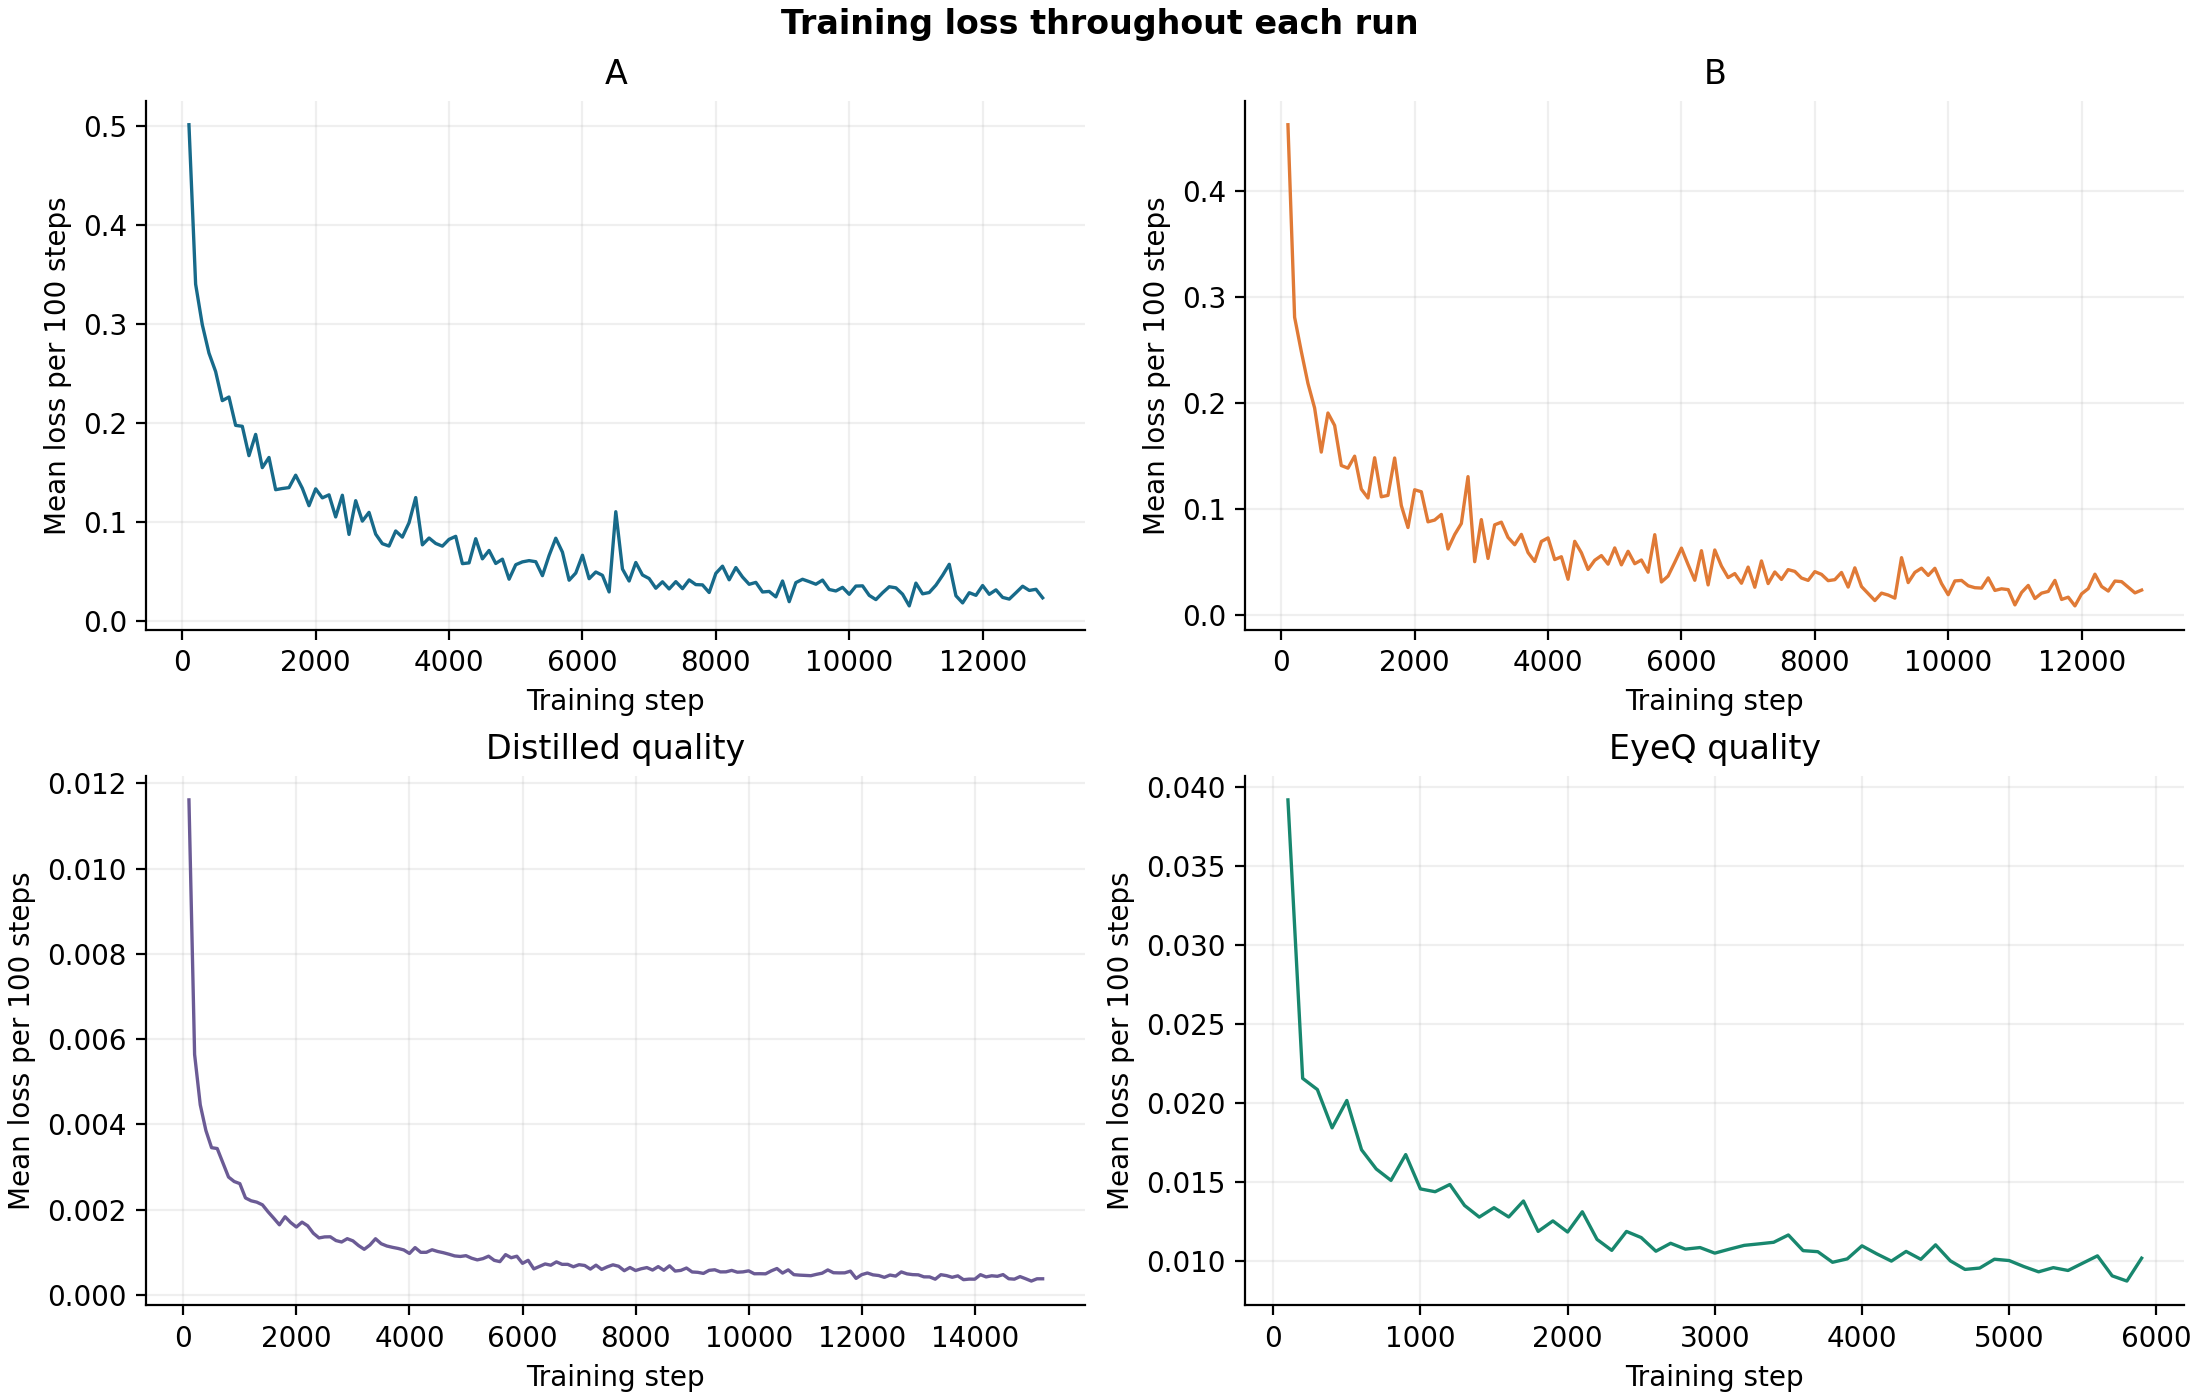
\includegraphics[keepaspectratio,alt={Training loss by step}]{04_step_loss.png}}
\caption{Training loss by step}
\end{figure}

Each point is the mean loss across 100 consecutive steps. All four step logs are continuous and their recorded losses are finite.

\subsection{Glaucoma models}\label{glaucoma-models}

\begin{figure}[H]
\centering
\pandocbounded{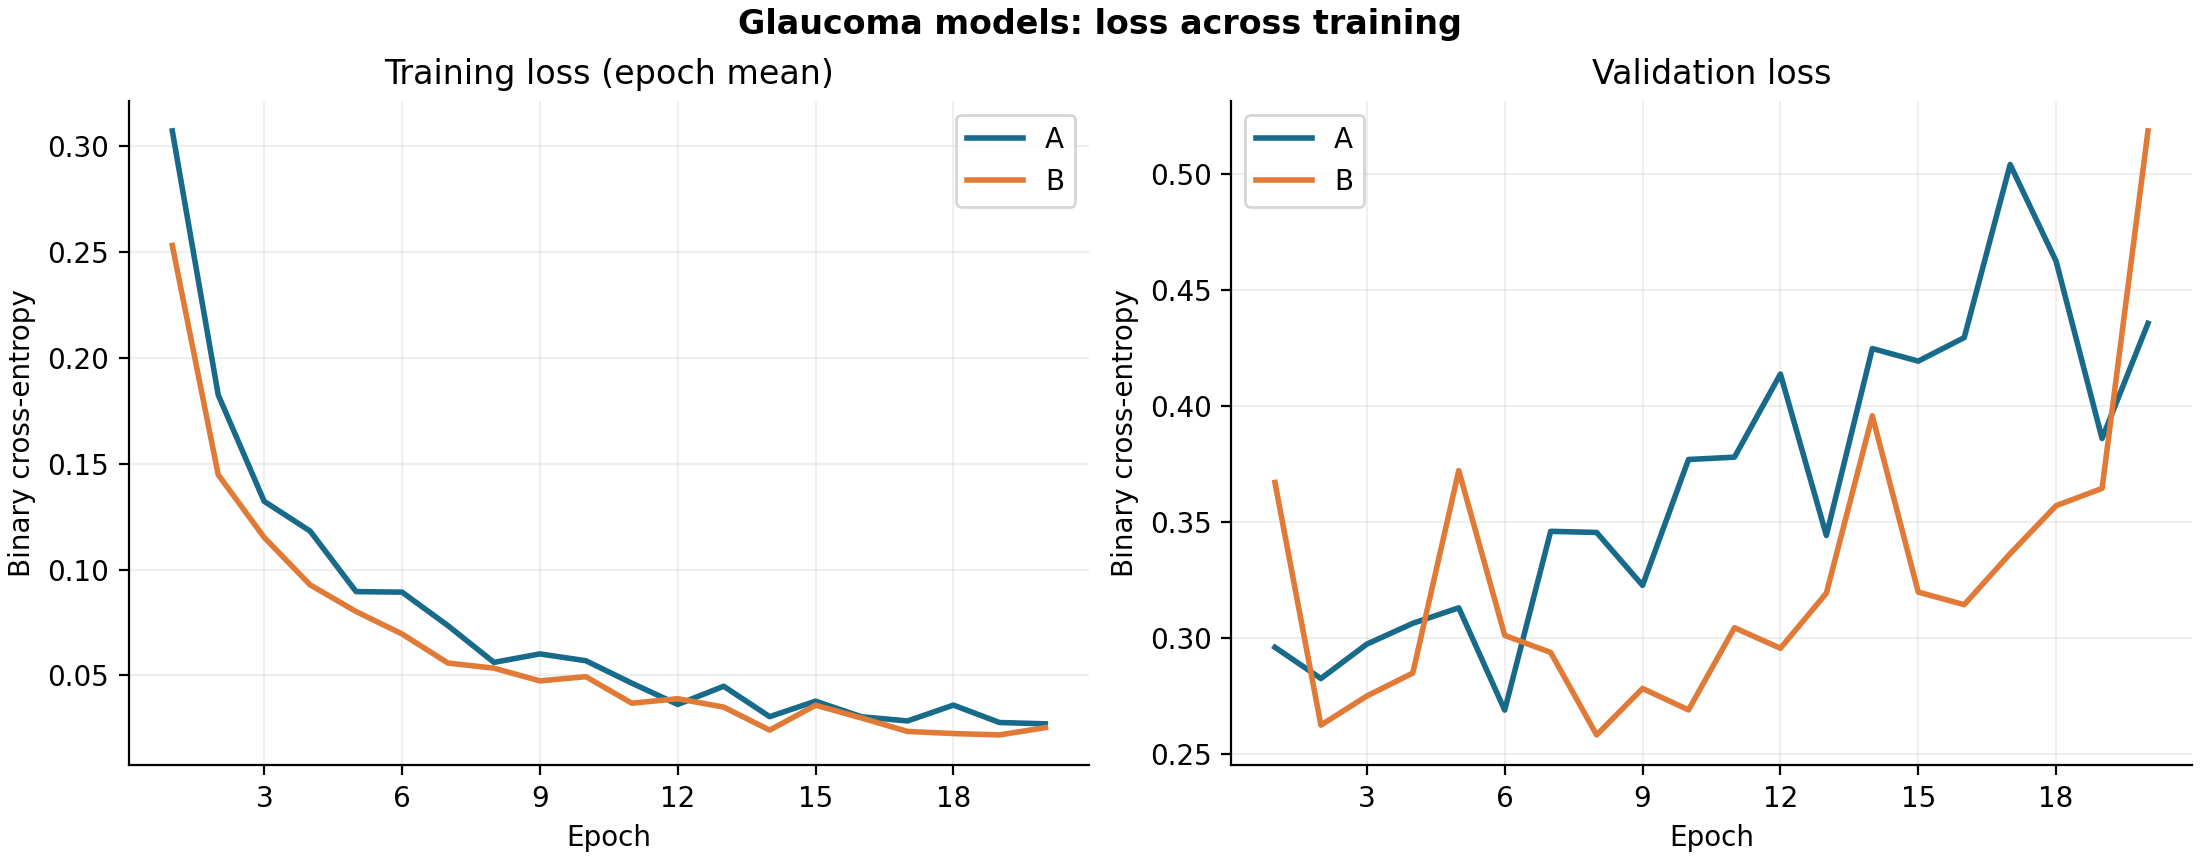
\includegraphics[keepaspectratio,alt={Glaucoma losses}]{01_glaucoma_loss.png}}
\caption{Glaucoma losses}
\end{figure}

Mean training loss fell from 0.307 to 0.027 for A and from 0.253 to 0.025 for B between the first and final epochs. Overall validation loss rose from 0.296 to 0.435 for A and from 0.367 to 0.518 for B. This divergence warrants a closer look at overfitting and probability calibration. Training curves show the arithmetic mean of batch losses within each epoch.

\begin{figure}[H]
\centering
\pandocbounded{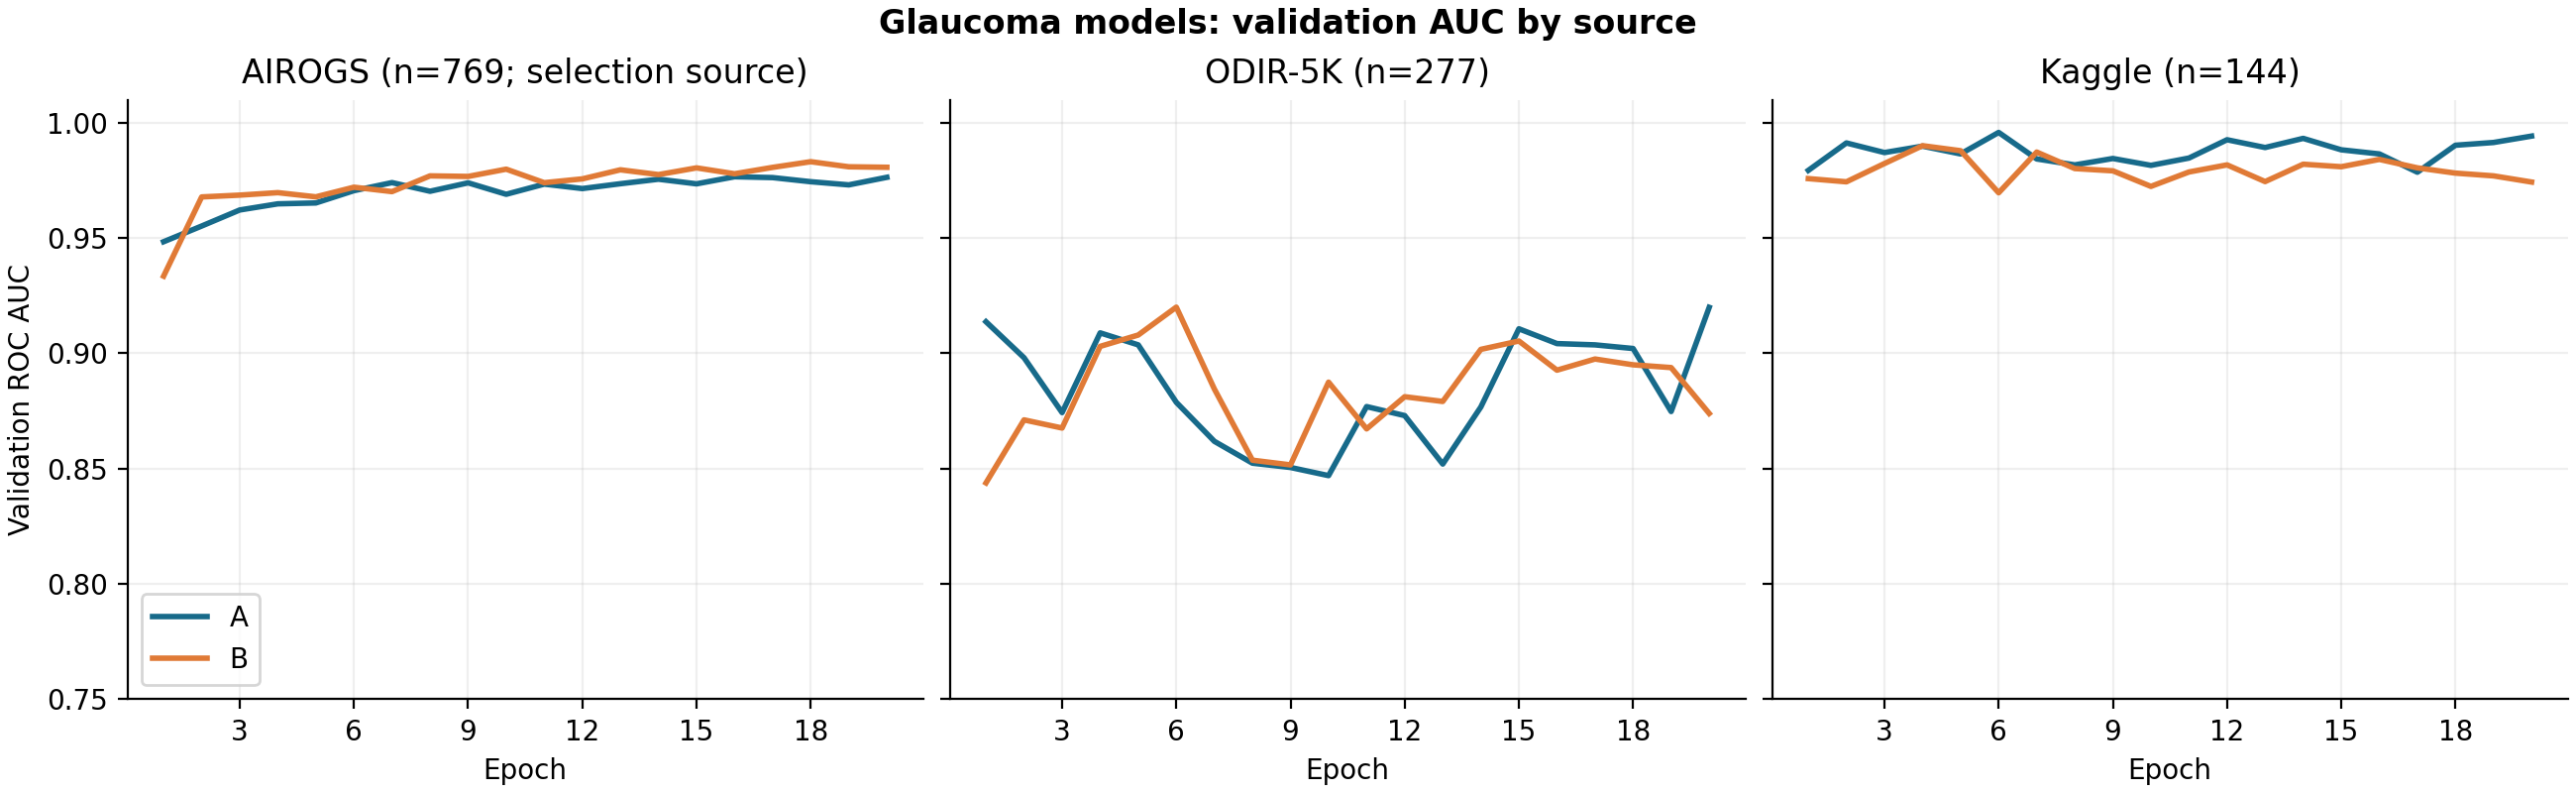
\includegraphics[keepaspectratio,alt={Validation AUC by source}]{02_glaucoma_auc.png}}
\caption{Validation AUC by source}
\end{figure}

AUC measures how well the model ranks positive cases above negative cases, without selecting a classification threshold. The AIROGS validation subset (769 images) was used to select checkpoints: A reached its best AUC of \textbf{0.9766 at epoch 16}, and B reached \textbf{0.9831 at epoch 18}. At epoch 20 the values were 0.9764 and 0.9807, respectively. ODIR-5K and Kaggle validation subsets contain 277 and 144 images.

The disease-model logs do not contain accuracy for each epoch. The prediction file is overwritten at each validation, so it represents the last validation, not every epoch or the selected checkpoint.

\subsection{Image quality models}\label{image-quality-models}

\begin{figure}[H]
\centering
\pandocbounded{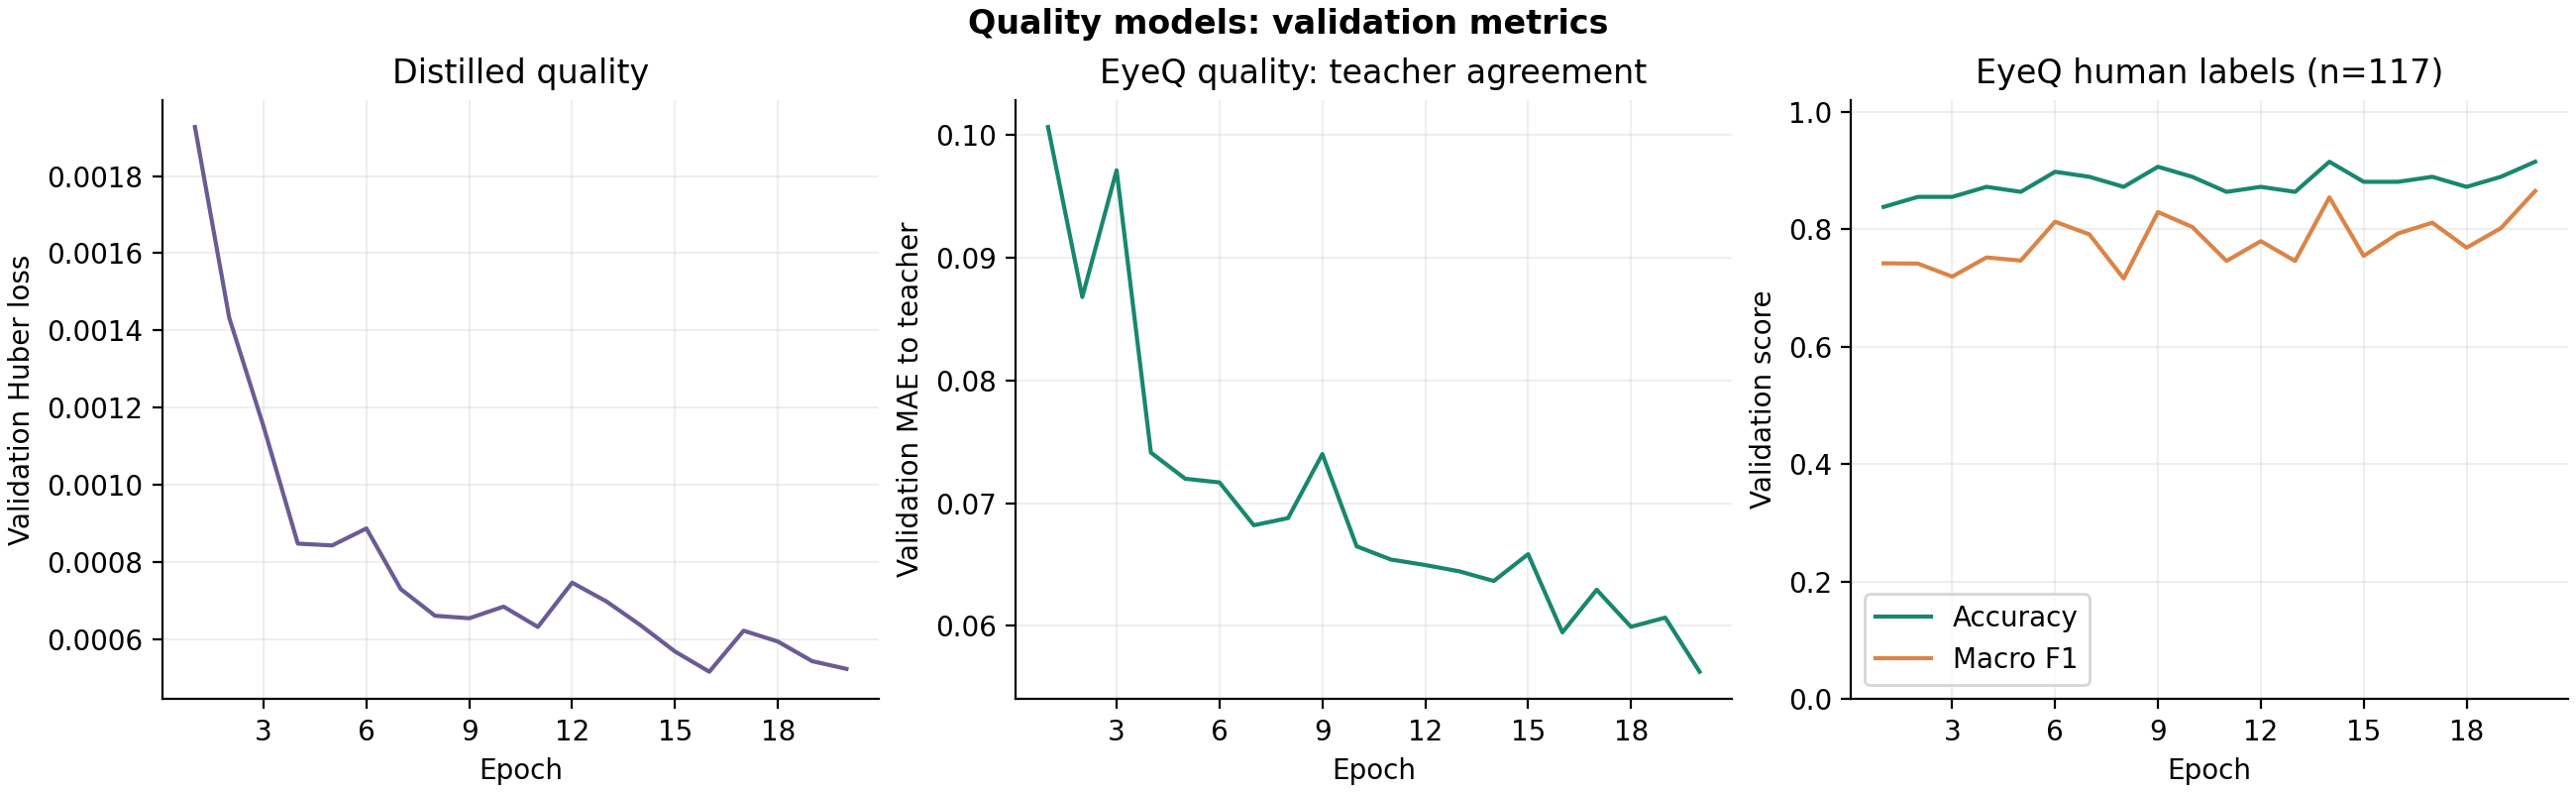
\includegraphics[keepaspectratio,alt={Quality validation measures}]{03_quality_validation.png}}
\caption{Quality validation measures}
\end{figure}

The original quality model's validation Huber loss fell from 0.001927 to 0.000524; its minimum was 0.000517 at epoch 16. This model learns continuous scores from a teacher model. Its validation target is the teacher score.

The EyeQ model was validated on 616 images, including 117 with human grades in three categories. Accuracy calculated from the saved confusion matrices rose from \textbf{83.8\% (98/117)} at epoch 1 to \textbf{91.5\% (107/117)} at epoch 20. The final macro-F1 was \textbf{0.865}. Macro-F1 gives equal weight to the performance of each grade, even when the grade counts differ.

The selected EyeQ checkpoint is epoch 17, chosen using a combined teacher and human-grade validation loss. Its accuracy is \textbf{88.9\% (104/117)} and macro-F1 is \textbf{0.811}. It is a different checkpoint from the final epoch.

\begin{figure}[H]
\centering
\pandocbounded{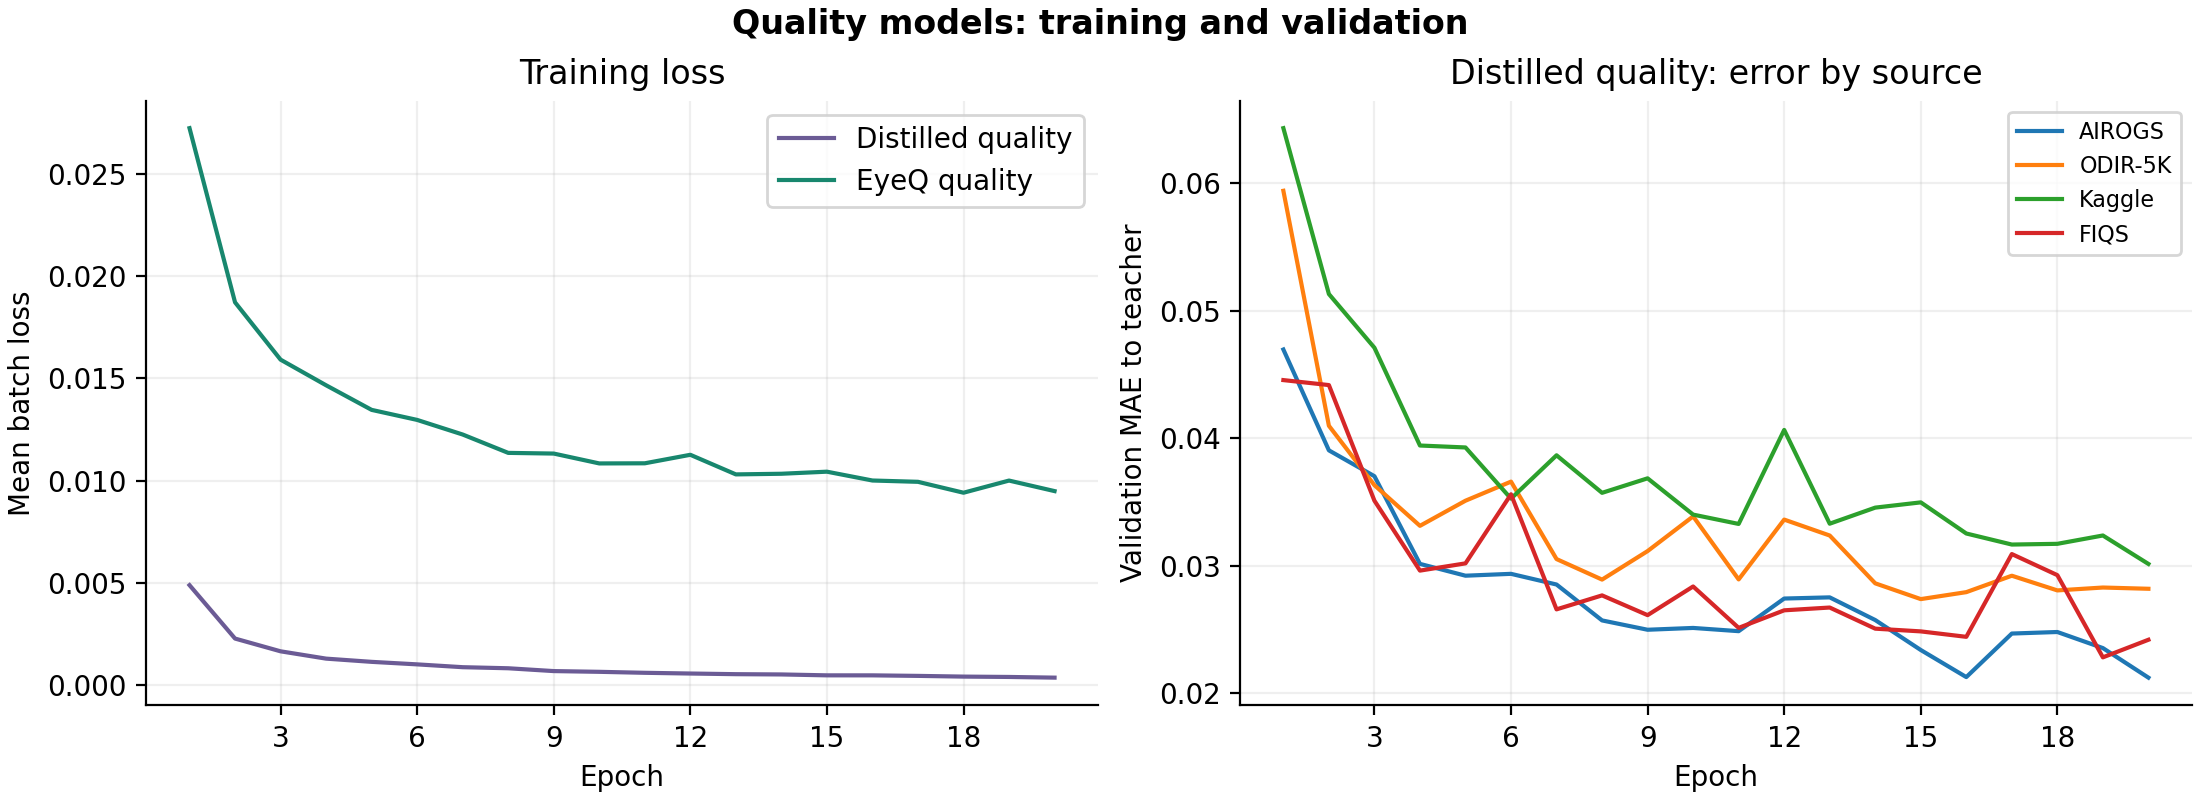
\includegraphics[width=0.88\linewidth,keepaspectratio,alt={Quality training and error by source}]{05_quality_detail.png}}
\caption{Quality training and error by source}
\end{figure}

The left panel shows each quality model's training loss. The right panel shows the original model's mean absolute difference from the teacher score by image source. Lower values indicate closer agreement with the teacher.

\begin{figure}[H]
\centering
\pandocbounded{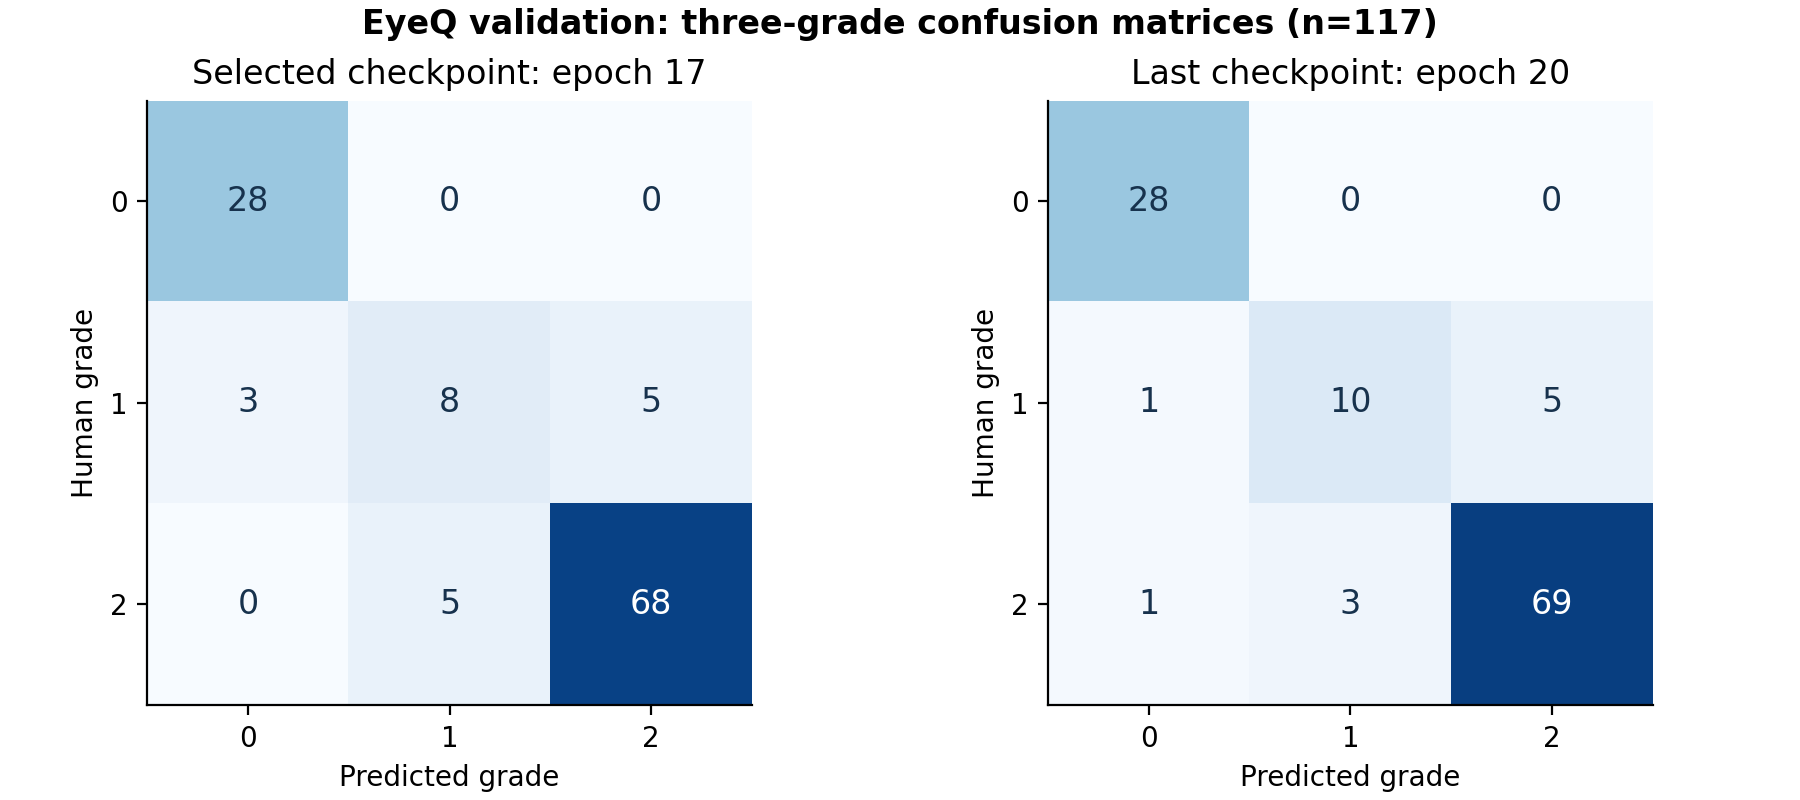
\includegraphics[width=0.88\linewidth,keepaspectratio,alt={EyeQ confusion matrices}]{06_eyeq_confusion.png}}
\caption{EyeQ confusion matrices}
\end{figure}

Rows show the human grade and columns show the predicted grade. The diagonal contains correct predictions. The left matrix is the selected checkpoint; the right matrix is the last epoch.

\subsection{Data and figure generation}\label{data-and-figure-generation}

The source records are the step and epoch logs, configurations, run summaries, and pipeline status files. The glaucoma and original quality model records are under \texttt{runs/formal\_v3/}; EyeQ records are under \texttt{runs/eyeq\_quality\_v1/quality\_student/}. In the original formal\_v3 logs, epoch numbers start at zero; the figures use 1--20. EyeQ validation logs already use 1--20.

The accompanying \texttt{chart\_data.json} contains step losses and aggregate validation metrics, without images or sample identities. Run \texttt{plot\_training.py} with Python and matplotlib to recreate the figures from this snapshot.

\end{document}
